%%%%%%%%%%%%%%%%%%%%%%%%%%%%%%%%%%%%%%%%%%%%%%%%%%%%%%%%%%%%%%%%%%%%%%
% Colorado State University LaTeX Thesis Template and Documentation
%
% by
%   Elliott Forney
%   2017
%
% This is free and unencumbered software released into the public domain.
% 
% Anyone is free to copy, modify, publish, use, compile, sell, or
% distribute this software, either in source code form or as a compiled
% binary, for any purpose, commercial or non-commercial, and by any
% means.
% 
% In jurisdictions that recognize copyright laws, the author or authors
% of this software dedicate any and all copyright interest in the
% software to the public domain. We make this dedication for the benefit
% of the public at large and to the detriment of our heirs and
% successors. We intend this dedication to be an overt act of
% relinquishment in perpetuity of all present and future rights to this
% software under copyright law.
% 
% THE SOFTWARE IS PROVIDED "AS IS", WITHOUT WARRANTY OF ANY KIND,
% EXPRESS OR IMPLIED, INCLUDING BUT NOT LIMITED TO THE WARRANTIES OF
% MERCHANTABILITY, FITNESS FOR A PARTICULAR PURPOSE AND NONINFRINGEMENT.
% IN NO EVENT SHALL THE AUTHORS BE LIABLE FOR ANY CLAIM, DAMAGES OR
% OTHER LIABILITY, WHETHER IN AN ACTION OF CONTRACT, TORT OR OTHERWISE,
% ARISING FROM, OUT OF OR IN CONNECTION WITH THE SOFTWARE OR THE USE OR
% OTHER DEALINGS IN THE SOFTWARE.
%%%%%%%%%%%%%%%%%%%%%%%%%%%%%%%%%%%%%%%%%%%%%%%%%%%%%%%%%%%%%%%%%%%%%%

% Preamble
%%%%%%%%%%%%%%%%%%%%%%%%%%%%%%%%%%%%%%%%%%%%%%%%%%%%%%%%%%%%%%%%

% use the thesis document class
% this is derived from the standard book class
% and supports many of the same features
\documentclass[master]{thesis}
%\documentclass[master,showframe]{thesis} % showframe helps troubleshoot margins
%\documentclass[doctor]{thesis} % for a dissertation
%\documentclass[bachelor]{thesis} % for an honor's thesis

% fonts
% use times font by default but you can choose a
% different font if you would like
%\usepackage{fourier} % fourier is also a nice choice

%\usepackage{helvet} % sans-serif helvetica works too
%\renewcommand\familydefault{\sfdefault}

% ams math packages
\usepackage[cmex10]{amsmath}
\usepackage{amsthm,amssymb}

% graphics packages
\usepackage[pdftex]{graphicx} % remove pdftex if you are not compiling to pdf
\graphicspath{{./figures/}} % this places all graphics in the figures subdirectory

% allowed graphics extensions
% uncomment if you prefer to add extension in \includegraphics
\DeclareGraphicsExtensions{.pdf,.png,.jpg}

% allows the creation of subfigures
\usepackage[caption=false]{subfig}

% book tables are simple and look nice
\usepackage{booktabs}

% for specifying urls and links
\usepackage{url}
\urlstyle{same} % same style as regular text

% for algorithms --- SIFAT
\usepackage[ruled]{algorithm2e}

% Additional commands
%%%%%%%%%%%%%%%%%%%%%%%%%%%%%%%%%%%%%%%%%%%%%%%%%%%%%%%%%%%%%%%%
\newcommand{\B}[1]{ \textbf{#1} }
\newcommand{\rmnum}[1]{\romannumeral #1}
\newcommand{\Rmnum}[1]{\expandafter\@slowromancap\romannumeral #1@}
%%%%%%%%%%%%%%%%%%%%%%%%%%%%%%%%%%%%%%%%%%%%%%%%%%%%%%%%%%%%%%%%




% Title Page
%%%%%%%%%%%%%%%%%%%%%%%%%%%%%%%%%%%%%%%%%%%%%%%%%%%%%%%%%%%%%%%%

% title of your thesis
\title{Revisiting Sparse Dynamic Programming\\ for the 0/1 Knapsack Problem}

% author's name
\author{Tarequl Islam Sifat}

% author's email address
\email{tarequl@colostate.edu}

% department name
\department{Department of Computer Science}

% semester of completion
\semester{Spring 2019}

% committee member names
\advisor{Sanjay Rajopadhye}
\coadvisor{Co-Advisor Name} % co-advisor is optional
\committee{Louisnoel Pouchet} % as many committee entries as you need
\committee{Edwin Chong}


% Copyright Page
%%%%%%%%%%%%%%%%%%%%%%%%%%%%%%%%%%%%%%%%%%%%%%%%%%%%%%%%%%%%%%%%

% here is an example of student copyright declaration
% note that the \copyright command prints the copyright symbol,
% so we use the name \mycopyright instead
\mycopyright{%
Copyright by Tarequl Islam Sifat 2018 \\
All Rights Reserved
}

% here is an example of a creative commons copyright license
% ask the graduate school for more information, if you are interested
%\mycopyright{%
%This work is licensed under the Creative Commons Attribution-NonCommercial-NoDerivatives 4.0 United States License.
%
%\vspace{3em}
%
%To view a copy of this license, visit:
%
%\vspace{2em}
%
%\url{http://creativecommons.org/licenses/by-nc-nd/4.0/legalcode}
%
%\vspace{3em}
%
%Or send a letter to:
%
%\vspace{2em}
%
%Creative Commons
%
%171 Second Street, Suite 300
%
%San Francisco, California, 94105, USA.
%}

% Abstract
%%%%%%%%%%%%%%%%%%%%%%%%%%%%%%%%%%%%%%%%%%%%%%%%%%%%%%%%%%%%%%%%

\abstract{%
  The 0/1-Knapsack Problem (KP) is a classic NP-hard problem, with two common
  approaches for solving it exactly: branch-and-bound (BB) and dynamic
  programming (DP).  A so called, ``sparse'' DP algorithm (SKPDP).  We first
  perform a careful empirical evaluation of SKPDP, and observe that for
  ``large enough'' capacity, $C$, the number of operations performed by SKPDP is
  invariant with respect to $C$.  This leads to the possibility of SKPDP
  providing an exponential improvement over the standard DP, comparable to what
  can be achieved by BB algorithms.

  DP algorithms have very regular structure and are amenable to highly parallel
  implementations.  We perform a roofline analysis of the sequential SKPDP, and
  show that it is memory bandwidth bound.  We develop two parallelizations
  (coarse-grain and fine-grain) of SKPDP on modern multicore processors (with
  $P$ cores).  We similarly analyze both parallelizations, and show that the
  coarse-grain version can reduce memory bandwidth requirements by a factor of
  $P$.  We expect the results of our ongoing experiments to validate these analyses.
}

% Acknowledgments 
%%%%%%%%%%%%%%%%%%%%%%%%%%%%%%%%%%%%%%%%%%%%%%%%%%%%%%%%%%%%%%%%

\acknowledgements{%
I would like to thank the CSU Graduate Student Council and the CSU Graduate School for initiating, commissioning and supporting this project.  I would also like to thank Nicole Ramo for her support and ensuring that we followed through with this project to completion.  I would like to thank Leif Anderson, who created and supported the previous LaTeX template for a number of years.  Although I have never met Leif, his work was invaluable in the creation of this package and has helped many students get their thesis approved by the CSU graduate school.  Finally, I would like to thank everyone who helps to contribute to this package.  Your work will help many CSU graduate students to create professional, beautiful and compelling theses and dissertations using LaTex.  Last but not least, thank you to the creators and maintaners of \LaTeX{} for creating a fantastic typesetting tool.
}

% Metadata
%%%%%%%%%%%%%%%%%%%%%%%%%%%%%%%%%%%%%%%%%%%%%%%%%%%%%%%%%%%%%%%%%%%%%%

% consider using hyperref to insert pdf metadata and make links clickable
% safe to remove if not using pdf or if it causes problems
\usepackage[pdfpagelabels,pdfusetitle,colorlinks=false,pdfborder={0 0 0}]{hyperref}

\begin{document} % preamble is complete, add any custom packages above
%%%%%%%%%%%%%%%%%%%%%%%%%%%%%%%%%%%%%%%%%%%%%%%%%%%%%%%%%%%%%%%%

\frontmatter % starts preliminary pages
%%%%%%%%%%%%%%%%%%%%%%%%%%%%%%%%%%%%%%%%%%%%%%%%%%%%%%%%%%%%%%%%

\maketitle              % insert title page
\makemycopyright        % insert copyright page
\makeabstract           % insert abstract page
\makeacknowledgements   % insert acknowledgements page

% any extra preliminary pages can be added here
% below is an example of a dedication page
% the dedication page is optional
\prelimtocentry{Dedication} % add table of contents entry
\begin{flatcenter} % center without extra space

    % page title
    DEDICATION

    %\vspace{3em} % place at top
    \vfill % or center on page

    \noindent \textit{I would like to dedicate this thesis to my dog fluffy.}
    \vfill % fill extra space at bottom
\end{flatcenter}
\newpage

\tableofcontents    % insert table of contents
\listoftables       % insert list of tables (optional)
\listoffigures      % insert list of figures (optional)

\mainmatter % starts thesis body

\chapter{Introduction}
\label{chap:intro}
%Many real-world applications have existing solutions that are NP-hard, which
%in worst case can be exponential in time complexity.
The 0/1 knapsack problem (0/1-KP, or just KP in this paper) is a well known,
NP-hard combinatorial optimization problem with applications in production
planning~\cite{Camargo-etal-COR-2012}, in risk balancing and assortment
optimization~\cite{Rooderkerk-vanHeerde-EJOR-2016}, and in storage capacity
limitation~\cite{Jolai-etal-AppMathComp-2007}.  It seeks to optimally fill a
knapsack of a given capacity, $C$, from a set of $N$ objects.  There are two
standard algorithmic approaches to solving it exactly: dynamic programming
(DP) and branch-and-bound (BB).  The execution time of BB may vary with
problem instances and this has led to very extensive research on techniques
and heuristics that work well in ``practice.''  On the other hand, most
standard implementations of DP build (at least conceptually) a table whose
size is parameterized by only the number of objects ($N$) and the capacity
($C$).  This leads to a complexity of $NC$, regardless of the specific
weight-profit distribution.  Most knapsack solvers therefore use DP only to
solve small knapsack sub-problems, leaving the ``heavy lifting'' to BB.
  
A so called, ``sparse'' DP algorithm (SKPDP) that performs fewer operations
than the standard algorithm (KPDP) is known for a while~\cite{sanjay-asap94,
  sanjay-irreg96} but to the best of our knowledge, there has been no
quantitative analysis of its benefits.  Moreover, the authors proposed a
``wavefront array'' (an early form of application-specific hardware
accelerator) for this algorithm, but that too, was not actually implemented.

Because 0/1-KP is ultimately an NP-Hard problem, it should be (and is)
possible to generate pathological problem instances where no technique has
significant advantage, and the execution time is exponential in the size of
the input.\footnote{Note that one of the inputs to the KP is the integer $C$,
  and its size, i.e., the number of bits needed to represent it, is $\lg C$.
  This is why an execution time proportional to $C$ is considered
  ``exponential.''}.

In this paper, we first do a careful experimental evaluation of the potential
benefits of SKPDP (see Section~\ref{sec:sparsity}).  We make the rather
surprising observation that when $C$ is sufficiently large, the expected
execution time (measured by counting the ``number of points generated'' by
SKPDP) becomes invariant with $C$, thereby providing a exponential gain due to
sparsity.

Next, we propose two parallelization techniques (see
Sections~\ref{sec:finegrain} and~\ref{sec:pipeline}) for implementing SKPDP on
modern multicore CPUs.  The first one is a fine-grain technique where
processors collaborate to compute the DP table, one row at a time.  In the
second, ``coarse-grain'' algorithm, the (virtual) processors operate in a
pipelined, ``producer-consumer'' fashion, each one responsible for computing
all the elements in a row.  We also do a detailed analysis of the two
algorithms identifying (i) the overheads of each scheme, and (ii) situations
when they are compute/memory bound.  This leads us to hypothesize that the
coarse grain parallelization is preferable in most situations.  We expect that
our (ongoing) experimental evaluation (Section~\ref{sec:expts}) will confirm
this, and expect to report it in a revised version of the paper.

% \begin{quote}
%   \textbf{\emph{This document is currently a place holder---a more complete
%       version of the paper is coming soon.}}
% \end{quote}

\chapter{Background}
\label{chap:background}
We now describe the background needed to make the paper self contained.  We
also present prior related work on the problem.

%\subsection{Dynamic Programming Solution of 0/1-KPDP}
% Taken From: 0/1 Knapsack on Hardware: A Complete Solution (Background section)

The 0/1 Knapsack Problem (KP) is formally
defined~\cite{Kellerer-etal-KP-book-2004} as follows.  Given a set of $N$
items, each  a known weight and a knapsack with a limited capacity $C$,
where each item $i$ consists of the profit $p_i$ and weight $w_i$ , the
objective of the 0/1-KP is to select items to achieve the maximum total profit
without exceeding the capacity.  Mathematically,

\begin{equation}
  \begin{array}{ll}
 \text{Maximize} & \quad {\displaystyle\sum^N_{i=1} p_i x_i} \\[5mm]
\text{subject to}& \quad {\displaystyle\sum^N_{i=1} w_i x_i < C} \\
 & \quad x_i \in \{0,1\}
  \end{array}
\end{equation}

% The general dynamic programming approach to the knapsack problem is to
% construct a table that is as wide as the capacity of the knapsack, and as
% high as the cardinality of the set of items to choose from. Starting from
% the element of the table that corresponds to the first item and a capacity
% of 1, the table is completed by computing elements of the table according to
% the recurrence equation:

%\subsection{Existing algorithms for solving 0/1-KP}

There is a significant body of work on algorithms and tools for KP, many of
them described in standard textbooks~\cite{MT90, Hu-IPNF-book-1969,
  Kellerer-etal-KP-book-2004, Cormen-etal-Algorithms-2009}.  Being an NP hard
problem, many authors investigate heuristic and/or approximate algorithms,
with or without bounds on the approximations.  As for exact solutions, there
are two main algorithms: dynamic programming (DP) and branch-and-bound (BB).
We focus on DP, which may be defined via the following recurrence.
% First approach is to find the exact optimal solution which in worst case
% will always have exponential time complexity. And the second approach is to
% find approximate solutions that have significantly less time-complexity but
% will not find the optimal solution every time.  Depending on the real-world
% problem requirements either type of solution can be used.

% Among the exact optimal solutions Dynamic Programming(DP) and
% Branch-and-Bound(BB) solutions are widely known.

\begin{equation} \label{eq:KPDP}
  \begin{array}{l}
    f(i,j) =  \\
    \left\{
    \begin{array}{ll}
      0,  & \text{if } i=0 \text{ or }k=0\\
      f(i,j-1),        & \text{if } i>0 \text{ and } j<w_i\\
      \max(f(j,i-1),\\
      p_i + f(j-w_i , i-1))   & \text{if } i>0 \text{ and } j \geq w_i
    \end{array} \right.
  \end{array}
\end{equation}

The function $f(i,j)$ denotes and defines the maximal profit that can be
achieved with a knapsack of capacity $j$, drawing items out of only the first
$i$ items.  The standard KPDP algorithm computes and stores this table in an
order (possibly in parallel) ditated by the dependences of the recurrence
doing $O(NC)$ work, and then performs an $O(N)$ work ``backtracking''
traversal of the table in order to construct the actual solution.  The total
execution time of KPDP is thus $O(NC)$

In this paper, we exploit two known improvements to KPDP.  The first one
reduces the space complexity to only $O(C)$ so that the whole table does not
need not be saved (this comes with a two-fold increase in execution time). For
the sake of completeness, we describe them here.

\section{Memory efficient KPDP}

The dynamic programming algorithm normally requires the entire table to be
retained, and this is often unaccpetably large for large problems.  The memory
efficient KPDP is an adaptation of an old trick to improve DP algorithms, that
was first proposed by Hirshberg for the longest common subsequence (LCS)
problem~\cite{Hirschberg-CACM-1975}.  The technique, described by Kellerer et
al.~\cite[pp 46-50]{Kellerer-etal-KP-book-2004} and by Nibbelink et
at.~\cite{sanjay-asap07} who also propose a hardware implementation on FPGAs,
avoids backtracking by recursively, \emph{directly solving} subproblems of the
form $\langle i, j, c \rangle$, that determine the optimal subset of the
$i$-through-$j$-th (inclusive) objects for a capacity of $c$.  The top level
call is thus to $\mathbf{Solve} \langle 1, N, C \rangle$, and
$\mathbf{Solve} \langle i, j, c \rangle$ proceeds as follows:

\begin{enumerate}
\item \textbf{Base case:} if $i=j$, there is only one object, so choose it if
  and only if it fits (i.e., $w_i\leq c$)
\item \textbf{General case:} Let $m=\lfloor\frac{j-i}{2}\rfloor$.  Determine
  (details below) a $c^*$ between 0 and $c$ such that in the (some) solution
  to the subproblem $\langle i,j,c\rangle$ the combined sum of the weights of
  the selected object in the ``first half'' i.e., $i$-through-$m$-th objects,
  is $c^*$.  This is called the ``optimal split'' of the capacity $c$.  Now,
  \begin{enumerate}
  \item Recursively call $\mathbf{Solve} \langle i, m, c^* \rangle$, and
  \item Recursively call $\mathbf{Solve} \langle m+1, j, (c-c^*) \rangle$
  \end{enumerate}
\end{enumerate}

So the main issue is to determine $c^*$.  We first determine for the first
``half'' of the objects, a vector $X[j]$ for $0\leq j\leq c$, the optimal
profit that can be obtained with capacity $j$ (using only objects in that
half).  We also construct a similar vector, $X'[j]$ for the other half.  This
can be done in only $2c$ memory using recurrence~(\ref{eq:KPDP}), by maintianing
only two rows of the table, and costs $(j-i)c$ work.  Using these two arrays,
$c^*$ is given by
\[ c^* = \mathrm{argmax}_{i=0}^{c} X[i]+X[c-i]
\]

The capacity arguments in all the calls at any levels of the recursion tree
add up to $c$, and the number of objects considered halves level by level.
Hence, the total work of this algorithm is $2NC$, just a two-fold increase.

% \begin{flushleft}
% \noindent\rule{9cm}{1pt}
% \textbf{Algorithm 1} Classic Backtracking
% \noindent\rule{9cm}{1pt}
% \end{flushleft}
% \begin{algorithmic}
% \STATE $cap = C; i = N$
% \WHILE {$i > 0$}
% 		\STATE $bitV ector = booleanT able[cap]$
% 		\STATE MASK OUT rightmost [$(i + 1)$to $N$ ] bits of $bitVector$
% 		\STATE $i$ = index of rightmost 1 bit in ( MASKED ) $bitVector$
% 		\STATE add $i$ to solution list
% 		\STATE $i = i - 1$
% 		\STATE $cap = cap - Weight[i]$
% \ENDWHILE
% \end{algorithmic}
% \noindent\rule{9cm}{1pt}

\section{Sparse KPDP (SKPDP)}

Andonov and Rajopadhye~\cite{sanjay-asap96} and Dupont de Dinechin et
al.~\cite{sanjay-irreg96} showed how, for the 0/1-KPDP and the UKP (the
unboundend knapsack problem), the sequences representing the $i$-th row could
be computed for the one representing the $(i-1)$-th row.  The work is similar
to early ideas on a list based algorithm~\cite{Horowitz-Sahni-JACM-1974} that
reduced the complexity of the subset-sum problem to $O(\sqrt{2^N})$, but uses
\emph{streams} of \emph{index-value pairs}.  The main idea behind the SKPDP is
the notion of monotomicity: it is clear that for any fixed $i$, the values of
$f(i,j)$ are monotomically non-decreasing with respect to $j$.  This is
because, in any subptooblem, we can do no worse than we are currently doing by
increasing capacity.  This is illustrated in Table~\ref{tab:sparsity1} which
shows the DP table for a KP instance where the four items have weights,
$5, 4, 6, 1$ and profits, $7, 8, 9, 4$, respectively.  The boxed entries are
the first occurrence of a value in a given row.  Because of sparsity, one may
enviage a ``sparse'' representation, where all the table entries are not
computed, rather only the ``points of inflection'' are explicitly evaluated.
To do this, we use a representation for the table in the form of
``index-value'' pairs: the entire $i$-th row is represented by a list, of the
form, $\langle j, f(i,j)\rangle$, as shown in Table \ref{tab:sparsity2}.

\begin{table}[htbp]
\caption{A 0/1-KPDP Table}
\begin{center}
\begin{tabular}{*{12}{|c}|}
  \hline
  \textbf{Items}&\multicolumn{10}{|c|}{Capacity} \\
  \cline{2-12} & \B{0} & \B{1}& \B{2}& \B{3}& \B{4}& \B{5}& \B{6}& \B{7}& \B{8}& \B{9}& \B{10} \\
  \hline
  \textbf{1}& 0 & 0& 0& 0& 0& \boxed{7}& 7& 7& 7& 7& 7 \\
  \hline
  \textbf{2}& 0 & 0& 0& 0& \boxed{8}& 8& 8& 8& 8& \boxed{15}& 15 \\
  \hline
  \textbf{3}& 0 & 0& 0& 0& \boxed{8}& 8& \boxed{9}& 9& 9& \boxed{15}& \boxed{17} \\
  \hline
  \textbf{4}& 0 & \boxed{4}& 4& 4& \boxed{8}& \boxed{12}& 12& \boxed{13}& 13& \boxed{15}& \boxed{19} \\
  \hline
\end{tabular}
\label{tab:sparsity1}
\end{center}
\end{table}

\begin{table}[htbp]
\caption{A SKPDP Table}
\begin{center}
\begin{tabular}{|c|l|}
\hline
\textbf{Items}& \\
\hline 
  \textbf{1}& $\langle 0, 0\rangle$, $\langle 5, 7\rangle$  \\
  \hline
  \textbf{2}& $\langle 0, 0\rangle$, $\langle 4, 8\rangle$, $\langle 9, 15\rangle$ \\
  \hline
  \textbf{3}& $\langle 0, 0\rangle$, $\langle 4, 8\rangle$, $\langle 6, 9\rangle$, $\langle 9,
              15\rangle$, $\langle 10, 17\rangle$ \\
  \hline
  \textbf{4}& $\langle 0, 0\rangle$, $\langle 1, 4\rangle$, $\langle 4, 8\rangle$, $\langle 5,
              12\rangle$, $\langle 7, 13\rangle$, $\langle 9, 15\rangle$,
              $\langle 10, 19\rangle$ \\
  \hline
\end{tabular}
\label{tab:sparsity2}
\end{center}
\end{table}

\section{Add-Merge-Kill}
\label{sec:merge-kill}
Andonov and Rajopadhye~\cite{sanjay-asap96} and Dupont de Dinechin et
al.~\cite{sanjay-irreg96} proposed to implementat the SKPDP algorithm on an
early form of hardware accelerator called a WAP (Wavefront Array
Processor~\cite{kung-sy-vlsi, kung-sy-etal}).  However, because the memory
efficient technique had not been discovered at that time, it remained an
unrealisitic paper design, because the total number of data transfers that the
accelerator needed to perform was the same order as the number of
computations.

The technique Add-Merge-Kill (AMK) is the core of SKPDP that generates the sparse table row-by-row. Let's take the 3\textsuperscript{rd} row of the Table (\ref{tab:sparsity2}),
\begin{equation}
\label{eq:list1}
\langle 0, 0\rangle, \langle 4, 8\rangle, \langle 6, 9\rangle, \langle 9, 15\rangle, \langle 10, 17\rangle
\end{equation}

This list of pairs (sparse row) is representative of the 3\textsuperscript{rd} row of the Table (\ref{tab:sparsity1}), that represents the maximum profits of taking the first 3 elements of the problem instance given capacities ranging from $1$ to $10$. From the 3\textsuperscript{rd} row to generate the 4\textsuperscript{th} row that also takes the 4\textsuperscript{th} element of the problem instance into consideration we first add the the weight and profit of the 4\textsuperscript{th} element, i.e. $\langle 1,4 \rangle$, to each pairs of the list (\ref{eq:2}).
We get,
\begin{equation}
\label{eq:list2}
\langle 1, 4\rangle, \langle 5, 12\rangle, \langle 7, 13\rangle, \langle 10, 19\rangle, \langle 11, 21\rangle
\end{equation}

Now applying the algorithm \ref{algo:MK} below to the lists (\ref{eq:list1}) and (\ref{eq:list2}) to get the 4\textsuperscript{th} row. 

\begin{equation}
\label{eq:list3}
\langle 0, 0\rangle, \langle 1, 4\rangle, \langle 4, 8\rangle, \langle 5,
              12\rangle, \langle 7, 13\rangle, \langle 9, 15\rangle,
              \langle 10, 19\rangle
\end{equation}

\begin{algorithm}

\SetAlgoLined
\KwResult{(i+1)-th row: $S_{i+1}$}
 $S_{i} \leftarrow $ current row\; 
 $S_{i+1} \leftarrow $ empty\;
 $S'_{i} \leftarrow $ $\langle weights[i], profits[i] \rangle$ added to each pairs of $S_i$\;
 $j,k,p \leftarrow 0,0,0$\;
 \While{the end of $S_i$ not reached}{
  \uIf{$S_i[j].weight < S'_i[k].weight$}{
   	\eIf{$S_i[j].profit < S'_i[k].profit$}{
   		$S_{i+1}[p] \leftarrow  S_i[j]$\;
   		$p \leftarrow p+1$\;
   		$j \leftarrow j+1$\;
   	} 	
	{
   		$k \leftarrow k+1$\;   	
   	}
   }
   \uElseIf{$S_i[j].weight > S'_i[k].weight$}{
   	\eIf{$S_i[j].profit > S'_i[k].profit$}{
   		$S_{i+1}[p] \leftarrow  S'_i[k]$\;
   		$p \leftarrow p+1$\;
   		$k \leftarrow k+1$\;
   	} 	
	{
   		$j \leftarrow j+1$\;   	
   	}
  }
  \Else{
   	\eIf{$S_i[j].profit > S'_i[k].profit$}{
   		$k \leftarrow k+1$\;
   	} 	
	{
   		$j \leftarrow j+1$\;   	
   	}  	
  }
 }
 \caption{Merge-Kill \label{algo:MK}}
\end{algorithm}





\chapter{Empirical Analysis of Complexity}

\label{chap:analysis}

\section{Generation of Problem Instances}

There has been extensive research on synthesis of knapsack problem instances. Pisinger \cite{Pisinger:2005:HKP:1063636.1063640} explored knapsack problem instances on several popular algorithms and showed that problem instances with strongly-correlated weights and profits are hardest problems to solve. To properly analyze SKPDP it's important to make sure that the knapsack problem instances that we use are not contrived and covers the input domain. We also have to generate the problem instances systematically when we are trying to analyze the impact of a particular attribute (i.e. correlation between weight and profit values) of problem instances on SKPDP. The attributes of the problem instances that we mainly focus on are, 

\begin{itemize}
\item The portion of the items that fit into the capacity
\item The distribution of the weights
\item The correlation between the weights and profits
\end{itemize}

We discuss this attributes in more details below.
\subsection{The portion of the items that fit into the capacity}
Before generating the problem instances for range of $N$ and $C$ values, we must decide how many items out $N$ should fit into the capacity $C$. If we decide that half of the items ($N/2$) should fit into the capacity then the average weight of all the items should be,
\[
W_{avg} = \frac{2C}{N}
\]

\subsection{The distribution of the weights}
Once we have the average weight ($W_{avg}$) we need to take a distribution of the weights. We used two different types of distribution. First, we used normal distribution with a mean of $W_{avg}$ and standard deviation of $0.3$. We also used a log-normal distribution with a mean of $W_{avg}$ while making sure that the largest weight ($W_{max}$) is close to $C$. This is to analyze the impact of very large weights on SKPDP.

\subsection{The correlation between the weights and profits}
When the ratio of weights and profits of all the items of knapsack problem is a constant we end up with the hardest problem instance. It essentially becomes a subset-sum problem. We want to see the impact of correlation between weights and profits on SKPDP. So, we generated problem instances with different levels of correlation between weights and profits. For that purpose we set the profits to be a constant factor larger than the weights and introduce a small noise value. The noise is used to adjust the correlation between the weights and profits.
\[
profit = alpha * weight + \text{ random integer in the range } [-noise*W_{avg},noise*W_{avg}]
\]









\section{Potential Gain}
We explore the computational gain of the SKPDP over the conventional 0/1-KPDP.
For SKPDP to be useful, the number of operations done by the sparse algorithm
must be significantly less that the dense version.  The number of iterations
needed to generate one row of the sparse table is equal or less than twice the
size (number of pairs) of the previous row.  So, the total number of
operations needed to generate the whole sparse table is a constant factor of
the total number of pairs/critical points in the generated sparse table.  The
more sparse the sparse table is for a certain problem instance the more
performance gain we can expect.  We define potential performance gain as,

\begin{align}
  \label{eq:2}
  \text{gain} &= 1 - \frac{\text{no.\ of iterations needed for
                SKPDP}}{\text{no.\ of iterations needed for 0/1-KPDP}}
                \nonumber \\
              &\approx 1 - \frac{\text{no. of iterations needed for
                SKPDP}}{2NC} \\
  [\text{because}&\text{, we are using memory efficient version of KPDP}]
                   \nonumber
\end{align}

Notice that according to (\ref{eq:2}), maximum performance gain we can
theoretically achieve is 1, positive values of gain implies that SKPDP should
perform better than conventional 0/1-KPDP and negative values of gain implies
that SKPDP should perform worse that conventional 0/1-KPDP.

In figure \ref{fig:gain1} we plot potential gain against problem instances
with capacity ranging from $2^{12}$ to $2^{30}$ and number of items ranging
from $2^7$ to $2^{12}$.  Please note that to generate the plot we used
$(18*5=)\ 90$ different 0/1-Knapsack problem instances each with items having
strongly-correlated weights and profits; a log-normal distribution of the
weight/profit values and where approximately one-eighth of the items fit into
the capacity (i.e., average weight is $8N/C$).

\begin{figure}[htbp]
\centerline{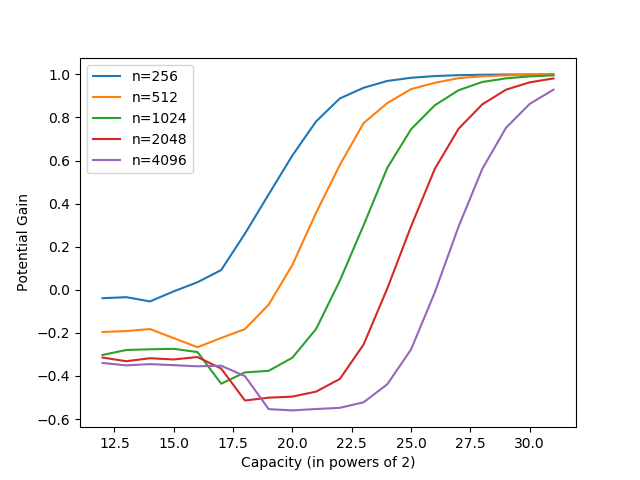
\includegraphics[width=.8\columnwidth]{images/gain1.png}}
\caption{Potential gain due to sparsity}
\label{fig:gain1}
\end{figure}

From the Figure \ref{fig:gain1} it is apparent that for large problems
instances (where capacity $C$ is much larger than $N$) we can expect
significant performance gain using SKPDP due to reduction in the number of
necessary computation to generate the sparse table.

\section{Empirical Results}
To prove our hypothesis that SKPDP performs significantly better for problem
instance where $N \ll C$ we do a log-log plot of the execution time vs the
capacity in Figure \ref{fig:time_vs_c1}.  Please note that the problem
instances in Figure \ref{fig:time_vs_c1} have the same attributes as of the
ones from the Figure \ref{fig:gain1}.  For problem instances with larger
capacity, the weight values are also proportionally larger to make sure that
the number of elements that fit into the capacity is constant for all problem
instances.  This is to make sure that our problem instances are not contrived.
 
\begin{figure}[htbp]
\centerline{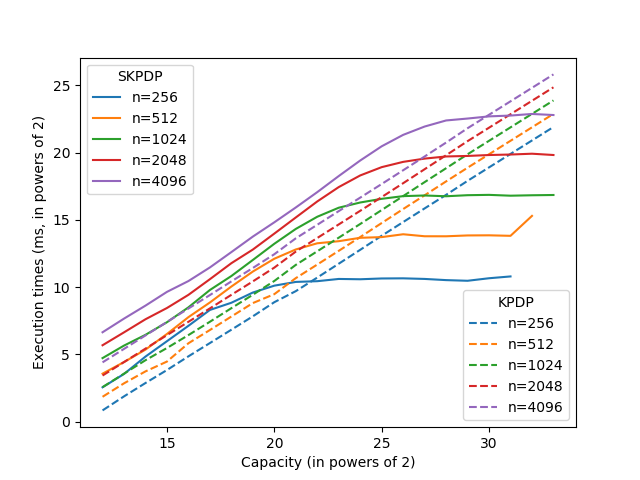
\includegraphics[width=.8\columnwidth]{images/time_vs_C1.png}}
\caption{Execution times of SKPDP for different instances of knapsack problem}
\label{fig:time_vs_c1}
\end{figure}


In the Figure \ref{fig:time_vs_c1}, the solid lines represent the execution times of SKPDP and the dashed lines represent the execution times of conventional 0/1-KPDP. We can observe that while the execution times of 0/1-KPDP stays linear with capacity $C$ (i.e. exponential with input size $log(C)$), the execution times of SKPDP becomes invariant with capacity. So, for problem instances where $N \ll C$, we can achieve exponential performance gain using SKPDP over 0/1-KPDP. SKPDP is a constant factor worse compared to 0/1-KPDP where $C$ is not large enough.

In the Figure \ref{fig:twin_vs_c1}, we can observe the correlation between the iteration count and execution time of our implementation SKPDP. It is apparent from the figure \ref{fig:twin_vs_c1} that the iteration count is correlated to the execution time of SKPDP.

\begin{figure}[htbp]
\centerline{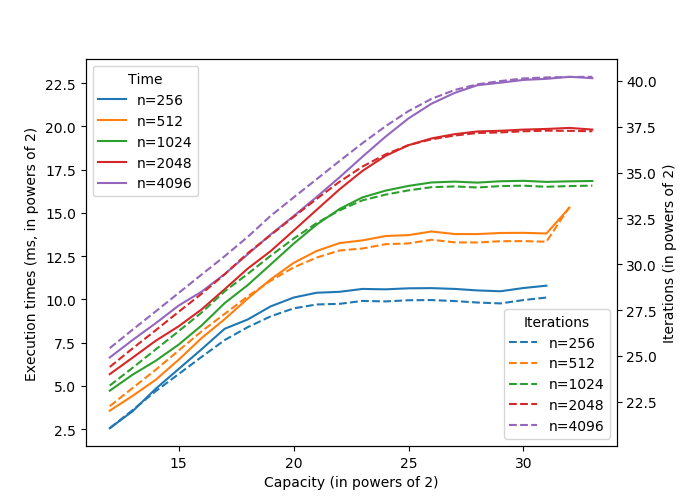
\includegraphics[width=.8\columnwidth]{images/twin_vs_C1.png}}
\caption{Comparing execution times and Op counts of SKPDP for different instances of knapsack problem}
\label{fig:twin_vs_c1}
\end{figure}

The question now is, how do we know if a problem instance has large enough value of $C$ for SKPDP to be useful over conventional KPDP? This threshold value depends on the number items ($N$), the correlation between the weights and profits and the amount elements fit into the capacity. 


\section{Impact of correlation of weights and profits}
The more strongly correlated the weights and profits of a knapsack problem instance are, the harder the problem instance is for any knapsack algorithm to solve. Figure \ref{fig:noise_vs_c1} shows that it is also true for SKPDP. When the weights and profits are perfectly correlated the SKPDP has exponential complexity. As we increase the noise value, thus reducing the correlation between weights and profits, we see much better performance by SKPDP. Note that the correlation of weights and profits does not impact the complexity of conventional 0/1-KPDP. On the other hand, even with fairly strong correlation between weights and profits we can see exponential performance improvement by SKPDP.

\begin{figure}[htbp]
\centerline{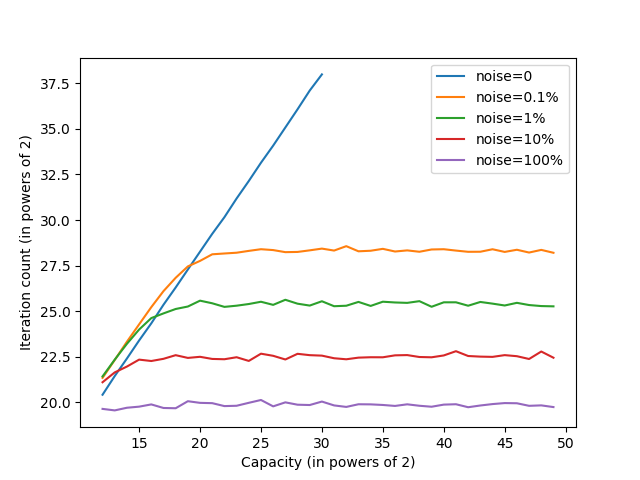
\includegraphics[width=.8\columnwidth]{images/noise_vs_C1.png}}
\caption{Iteration count of SKPDP for different levels of correlation between the weights and profits; For all problem instances $N = 256$ and $W_{avg} = \frac{8C}{N}$}
\label{fig:noise_vs_c1}
\end{figure}
\newpage



\section{Impact of the portion of items that fit into the capacity}
Figure \ref{fig:fits_vs_c1} compares the iteration counts of knapsack problem instances with 4 different average weights of the items. When we want half of the items to fit into the capacity (on average), we make sure that $W_{avg}=\frac{2C}{N}$; when we want 1/4-th of items to fit into the capacity, we make sure that $W_{avg}=\frac{4C}{N}$ and so on. From the figure \ref{fig:fits_vs_c1} it is apparent that for any given $N$ and $C$ values, problem instances with higher values of $W_{avg}$ have more sparsity. Again, note that this attribute does not impact the complexity of conventional 0/1-KPDP.


\begin{figure}[htbp]
\centerline{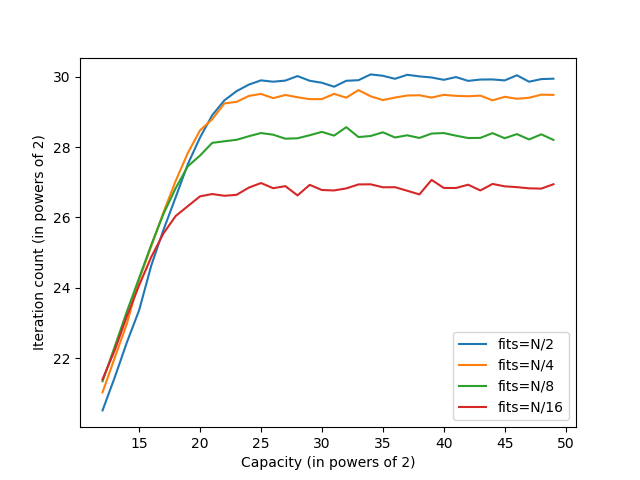
\includegraphics[width=.8\columnwidth]{images/fits_vs_C1.png}}
\caption{Iteration count of SKPDP for different portions of the items fitting into the capacity; For all problem instances $N = 256$ and $noise = 0.1\%$}
\label{fig:fits_vs_c1}
\end{figure}


\chapter{Fine-grain Parallelization}
\label{chap:finegrain}

%We explore two parallelization strategies, Coarse-grain and Fine-grain. In the Coarse-grain parallelization strategy, a processor is responsible for computing an entire row in the table.  Whereas in the Fine-grain parallelization strategy, all processors contribute to the computation of a row.

%\subsection{Coarse-grain Parallelization}
%ABCD

%\subsection{Fine-grain Parallelization}
In fine-grain parallelism, the computation of a single row is equally distributed amongst $P$ processors or threads (except the last processor which might have less number of elements to compute).  Every row in the sparse table has a different size.  If the size of the row is less than $P*W_{i}*\alpha$, then the row is computed by a single processor (or thread).  Here,  $\alpha$ is a constant greater than $2$.  Once the size of the row exceeds the threshold of $P*W_{i}*\alpha$, the row is equally split into $P$ sections with contiguous elements such that the $i_{th}$ processor is responsible for computing the $i_{th}$ section of the row.  The size of each section is $C/P$, where the last processor might have less number of elements to compute.  All processors independently compute their respective sections in parallel.  When all processors have finished computing, the sections are then stitched together using a mechanism similar to the \emph{Merge-kill} mechanism explained in section-----sectionNAME.  
%This stitching is performed by a single processor.  
Additionally, the elements are sorted by the decreasing order of their weights.  This means the element with maximum weight is computed first and the element with the minimum weight is computed at the end.  This allows for $P$ processors to start computing rows in parallel from a certain point in the table and continue parallel execution henceforth.  


\begin{figure}[htbp]
\centerline{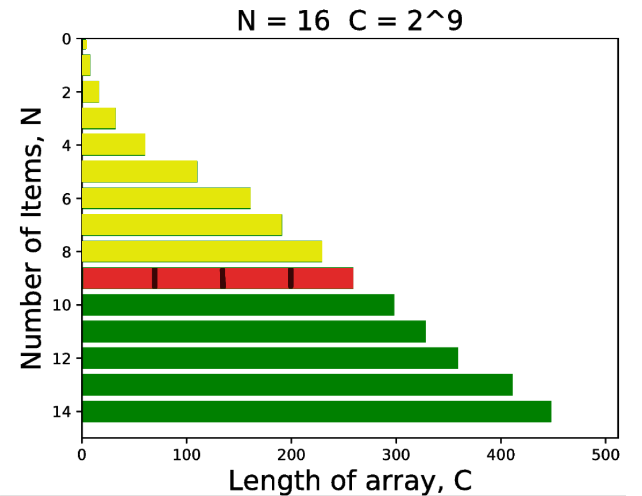
\includegraphics[width=1\columnwidth]{images/finegrain.png}}
\caption{Fine-Grain Parallelization. }
\label{fig:finegrain}
\end{figure}

As shown in Figure \ref{fig:finegrain}(a),  the fine-grain parallel computation begins at the red row where the size of the row is greater than $P*W_{i}*\alpha$.  The  row is split into $P$ sections, each section has a starting index and a ending index.  A processor (or a thread) computes its section while reading the elements from previous row and produces a current/output buffer.  All the threads execute in parallel and produce an output buffer.  These output buffers then have to be merged in order to produce the output row.  Note that some of the values produced by the output buffer of the processor $P_i$ may be dominated by the elements in the output buffer of the processor $P_{i+1}$. See Figure \ref{fig:finegrain} (b).  The suffix of the output buffer of the processor $P_i$ will have an overlap with the prefix of the output buffer of the processor $P_{i+1}$.  The output buffers therefore need to be stitched together and more work is needed.  For the stitching, all the threads (in parallel) eliminate dominating values from their suffix and produce a merged output row.  The threads move on to the next row after stitching.

\paragraph{Overhead Analysis} The extra work involved in the stitching can slow down the computation.  The maximum overlap between any two threads can be of the size of $W_i$\footnote{Note that the size of the row must be greater than $P*W_{i}*\alpha, \alpha>2$.  This ensures that there cannot be any overlap between the processors $P_{i-1}$ and $P_{i+1}$.}.  In the worst case, $W_i$ elements will need to be merged for every section for every row.  This means that a total of $P* \sum_i W_i$ extra computation must be performed for stitching the output row.  The upper bound on $P* \sum_i W_i$ is $C$, the capacity.  Every row will do $C$ extra work, at worst.  This means a total of $N*C$ extra work is done which is double the work compared to sequential version.


\chapter{Parallelization using Pipelining Technique}
\label{chap:pipeline}

The conventional 0/1-KPDP lends itself to a very straight-forward parallelization, because any element of a certain row of the dense table can be calculated independently of other elements of the same row, given the previous row. On the other hand, to calculate a row of the sparse table in SKPDP we use a process called \textit{Merge-Kill} which is inherently sequential.

The idea of using the pipelining technique stems from the understanding that the whole row of sparse table does not have to be calculated before starting the calculation of the next row. So, as a row of the sparse table is being computed, the values can be used immediately for calculating the next row. This way each thread is responsible for calculating one row of the sparse table and each thread acts as a consumer of the values produced by the previous thread. In hardware this can be implemented as streaming input to processing elements --REFERENCE--, but in software synchronization between threads is costly. So to minimize synchronization cost between threads the data between two consecutive threads can be shared in blocks instead of one data-point at a time. The block size is a very important parameter to be tuned in this algorithm, because too large of block size hinders parallelism and too small of a block size introduces more synchronization cost between threads.

Note that using this technique we only completely write out every $p$-th row of sparse table into memory. So, the the $(p-1)$-th thread is responsible for maintaining a whole row, where the threads 0 to $p-2$ maintain a local buffer of size $w_i$. 


\begin{figure}[htbp]
\centerline{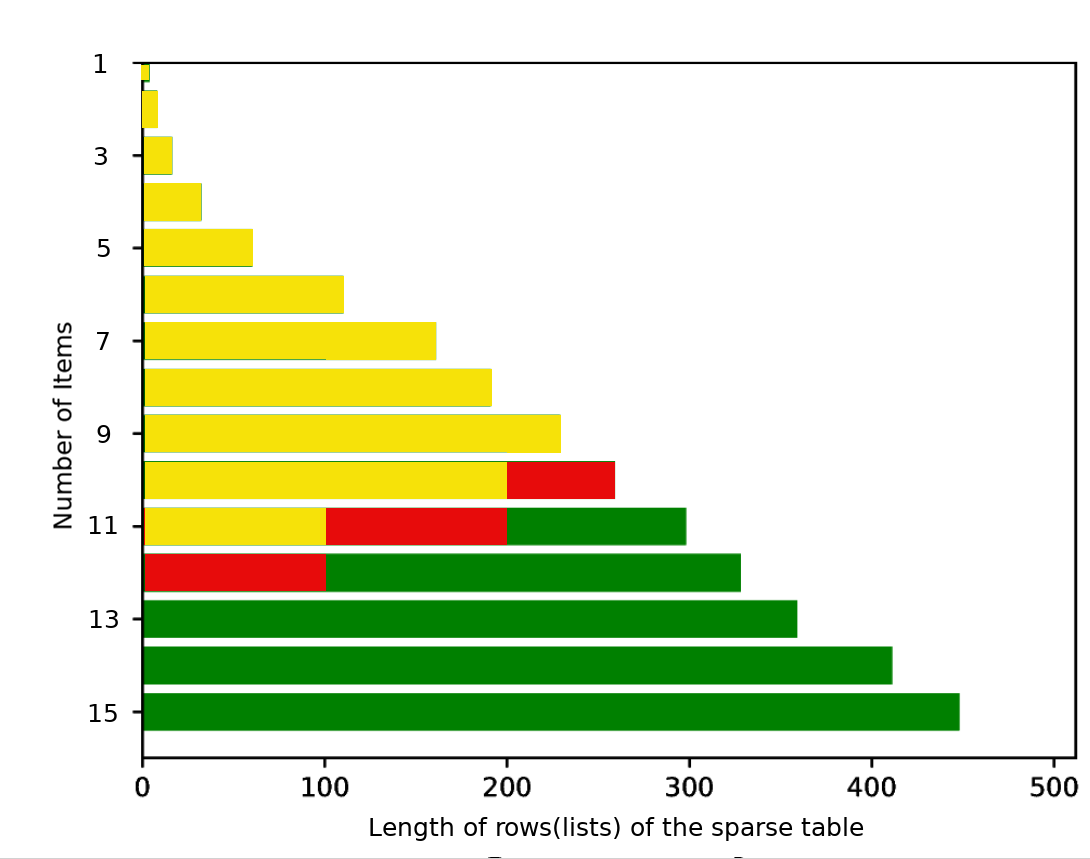
\includegraphics[width=1\columnwidth]{images/pipelining.png}}
\caption{Pipelining (coarse-grained) parallelism of KSPDP }
\label{fig:pipeline}
\end{figure}

Figure \ref{fig:pipeline} represents the idea of pipelining in the context of SKPDP. Let's take a small knapsack problem instance with $n=15$ and $C=512$ for demonstration purposes. The horizontal bars represents the size of each row of the sparse table. The yellow colored parts are already calculated; the red blocks are being calculated in parallel and the green parts are yet to be calculated.

\paragraph{Overhead Analysis} Most of the overhead of the computation comes from block synchronization and additional memory reads and writes of our current implementation which still requires some optimization. The space-complexity of this algorithm is $O(2nC + w_{max}p)$ because of the $p$ thread have to maintain a buffer of $w_i$.
\chapter{Implementation and Results}
\label{chap:implementation-results}

\section{Experimental Setup}
We do all our experiments on linux machines with \textit{Intel(R) Xeon(R) CPU E5-2650 v2} processors running at 2.60GHz with 32GB of RAM. The compiler used is \textit{Intel C++ Compiler} version 19.0.0.117. We used \textit{OpenMP } for implementing  prallelization on CPU.


\section{Implementation details of sequential implementation of SKPDP algorithm}
As we are not backtracking and instead using Divide and Conquer to find the complete solution, we allocate two arrays of pairs(critical points) of size $C$. Let, $(w_i,p_i)$ represent the weight and profit pair of the $i$-th element. We initially put $(w_0,p_0)$ into one of the allocated arrays. Then we apply the \textit{Add-Merge-Kill} process described in section --REFERENCE-- and store the output in the other allocated array. We iteratively find the last row of the sparse table.


\section{Implementation details of Fine-grained parallelization of SKPDP algorithm}
For this parallelism to be applicable on a row, the row must conform to the criteria below,

\begin{equation}
\label{eq: fine-grained-criteria}
l_{i-1} > \alpha P w_i
\end{equation}
where $l_{i-1}$ is length of the last calculated row, $\alpha$ is a parameter chosen to tune the parallelization strategy, $P$ is number of intended threads to be used (ideally equal to the number of processors) and $w_i$ is the weight of the current item to be taken into account for maximizing the total profit.

Topmost rows of the SKPDP are calculated exactly as the sequential version of SKPDP until (\ref{eq: fine-grained-criteria}) is true. All subsequent rows are computed in $P$ separate chunks on $P$ different processors. So, we allocate a total of $2P$ additional arrays of pairs(structures) of size $C$. When we split the calculation of a single row between multiple threads we end up generating some extra point at each thread. So, ones all the threads are finished computing their own chunk of a row, we do a barrier synchronization and run a process called stitching between the $P$ threads. Stitching gets rid of the points that are dominated by points in the adjacent chunk. There are $P-1$ different stitching points which can be run on parallel on $P-1$ different threads. The process of stitching between two threads takes $2w_i$ iterations in the worst case ($2P w_i$ for the whole $i$-th row).



\section{Implementation details of Coarse-grained/Pipelined of SKPDP algorithm}



[TODO]



\begin{table}[htbp]
\caption{Summery of our results}
\begin{center}
\begin{tabular}{|p{.23\columnwidth}|p{.23\columnwidth}|p{.23\columnwidth}|p{.23\columnwidth}|}	
\hline
\textbf{Implementation}& \textbf{Expectation} & \textbf{Observation} & \textbf{Reasoning} \\
\hline
\textbf{Sequential SKPDP} 
& Large problem instance with $N \ll C$ should show significant performance improvement over SKPDP.
& We observe exponential improvement of performance of SKPDP when $N \ll C$.
& Observation reflects our expectation.\\
\cline{2-4}
& Problem instance with stronger correlation between the wights and profits shows lowest sparsity.
& As the 0/1-knapsack gets closer to a Subset-Sum problem, we observe less sparsity.
& Observation reflects our expectation.\\
\cline{2-4}
& The ratio of elements that fit into the capacity on average may have impact in the sparsity.
& When the weights are relatively larger (less elements fit into the capacity) we observe more sparsity.
& Observation reflects our expectation.\\
\hline

\textbf{Fine-grained parallelization of SKPDP} 
& The overhead of stitching the separate parts could potentially nullify the benefits of parallelism.
& Observations so far proves our suspicion and the parallel version seem to perform a constant factor worse than the sequential version.
& As suspected the overhead of stitching  does seem to nullify the benefits of parallelism.\\
\cline{2-4}
& $W_i$ should be sorted in decreasing order to maximize parallelization.
& We do not observe expected performance gain, but this detail have important implications in our implementation.
& The reason for this is yet to be explored.\\
\cline{2-4}
& Top-most rows of the sparse table are too small to be parallelized using this method. The parameter $\alpha$ dictates when we start parallelizing (i.e. at what point a row of the sparse table becomes large enough to be parallelized). We must tune $\alpha$ perfectly for the best performance.
& Smaller value of $\alpha$ causes higher overhead of stitching and larger value of $\alpha$ cause most rows to be not palatalized at all.
& Observation does reflect our expectation.\\

\hline

\textbf{Coarse-grained/Pipelined parallelization of SKPDP} 
& Block size (i.e. number of data points shared between producer and consumer thread at one time) is significantly important parameter.
& Observation seem to verify our expectation and block size is an important tune-able  parameter for every problem instance.
& Too small of a block size causes more block synchronization overhead and too large of a block size hinders parallelism\\
\cline{2-4} 
& Optimal number of threads $P$ to be used should be the number of cores available in the system.
& We observe that we get better performance when the number threads $P$ is larger than the number of cores in the system.
& The reason for this is yet to be explored.\\
\cline{2-4} 
& We expect $P$ fold performance improvement.
& We never observe $P$ fold performance improvement and unlike the sequential version the performance does not seem to become invariant with capacity when $n \ll C$.
& In theory this implementation should not do exponentially worse than the sequential version. More experiments are needed to figure out the reason behind this phenomenon. \\
\hline




\hline
\end{tabular}
\label{tab:result-summery}
\end{center}
\end{table}
%%%%%%%%%%%%%%%%%%%%%%%%%%%%%%%%%%%%%%%%%%%%%%%%%%%%%%%%%%%%%%%%



\backmatter % starts unnumbered supplementary material
%%%%%%%%%%%%%%%%%%%%%%%%%%%%%%%%%%%%%%%%%%%%%%%%%%%%%%%%%%%%%%%%

% Bibliography
%%%%%%%%%%%%%%%%%%%%%%%%%%%%%%%%%%%%%%%%%%%%%%%%%%%%%%%%%%%%%%%%

% unsorted BibTeX style
% check here for more:  https://www.sharelatex.com/learn/Bibtex_bibliography_styles
\bibliographystyle{unsrt}
% \bibliography{sample} % change sample to the name of your .tex file, e.g., thesis
\bibliography{bib4,parallelizing,SKPDP}
\appendix % starts the appendices
%%%%%%%%%%%%%%%%%%%%%%%%%%%%%%%%%%%%%%%%%%%%%%%%%%%%%%%%%%%%%%%%

\chapter{License}
\label{appendix:license}
%%%%%%%%%%%%%%%%%%%%%%%%%%%%%%%%%%%%%%%%%%%%%%%%%%%%%%%%%%%%%%%%


% Have a nice day!
%%%%%%%%%%%%%%%%%%%%%%%%%%%%%%%%%%%%%%%%%%%%%%%%%%%%%%%%%%%%%%%%
\end{document}
